% !TEX root = ../../thesis.tex
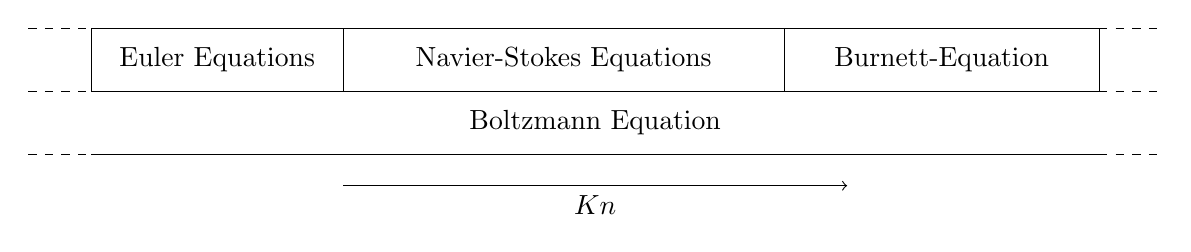
\begin{tikzpicture}[ scale=.8]

\draw[draw=white] (1,0) rectangle (17,-1) node[pos=0.5] {Boltzmann Equation};
\draw[style=dashed] (0,0) -- (1, 0);
\draw[style=dashed] (0,1) -- (1, 1);
\draw (1,0) rectangle (5,1) node[pos=.5] {Euler Equations};
\draw (5,0) rectangle (12,1) node[pos=.5] {Navier-Stokes Equations};
\draw (12,0) rectangle (17,1) node[pos=.5] {Burnett-Equation};
\draw[style=dashed] (17,0) -- (18, 0);
\draw[style=dashed] (17,1) -- (18, 1);

\draw (1,-1) -- (17, -1);
\draw[style=dashed] (0,-1) -- (1, -1);
\draw[style=dashed] (17,-1) -- (18, -1);
\draw (1,-1) -- (17, -1);

\draw[->] (5,-1.5) -- (13, -1.5) node[midway, below] {$Kn$};

\end{tikzpicture}
